\documentclass[12pt,a4paper]{article}

\usepackage[utf8]{inputenc}
\usepackage{ucs}

\usepackage[francais]{babel}

\usepackage{multicol}

\usepackage{color}
\usepackage{hyperref}
\hypersetup{
    colorlinks,
    citecolor=black,
    filecolor=black,
    linkcolor=black,
    urlcolor=black
}

\usepackage{ifplatform}

\usepackage[apmep, fr]{lyxam}

\usepackage{amssymb}
\usepackage{textgreek}
\usepackage[raggedright]{titlesec}

\titleformat{\paragraph}[hang]{\normalfont\normalsize\bfseries}{\theparagraph}{1em}{}
\titlespacing*{\paragraph}{0pt}{3.25ex plus 1ex minus .2ex}{0.5em}


\newcommand\ascii{\texttt{ASCII}}

\usepackage[utf8]{inputenc}
\usepackage{ucs}
\usepackage[top=2cm, bottom=2cm, left=1.5cm, right=1.5cm]{geometry}

\usepackage[francais]{babel}

\usepackage{color}
\usepackage{hyperref}
\hypersetup{
    colorlinks,
    citecolor=black,
    filecolor=black,
    linkcolor=black,
    urlcolor=black
}

\usepackage{multicol}
\usepackage{enumitem}

\usepackage{amsthm}

\usepackage{tcolorbox}
\tcbuselibrary{listingsutf8}

\usepackage{pgffor}
\usepackage{xstring}


% MISC

\tcbset{%
	sharp corners,%
	left=1mm, right=1mm,%
	bottom=1mm, top=1mm,%
	colupper=red!75!blue% 
}

\setlength{\parindent}{0cm}

\theoremstyle{definition}
\newtheorem*{remark}{Remarque}

\usepackage[raggedright]{titlesec}

\titleformat{\paragraph}[hang]{\normalfont\normalsize\bfseries}{\theparagraph}{1em}{}
\titlespacing*{\paragraph}{0pt}{3.25ex plus 1ex minus .2ex}{0.5em}

\makeatother
	\newcommand\resetallcnt{
		\setcounter{lyxam@counter@topic}{0}
		\setcounter{lyxam@counter@exercise}{0}
		\setcounter{lyxam@counter@problem}{0}
		\setcounter{lyxam@counter@bonus}{0}
		\setcounter{lyxam@counter@subpart}{0}
	}
\makeatletter

% Technical IDs

\newwrite\tempfile

\immediate\openout\tempfile=x-\jobname.macros-x.txt

\AtEndDocument{\immediate\closeout\tempfile}

\newcommand\IDconstant[1]{%
    \immediate\write\tempfile{constant@#1}%
}

\makeatletter
	\newcommand\IDmacro{\@ifstar{\@IDmacroStar}{\@IDmacroNoStar}}
	
    \newcommand\@IDmacroNoStar[3]{%
        \texttt{%
        	\textbackslash#1%
        	\IfStrEq{#2}{0}{}{%
        		\,\,[#2 Option%
				\IfStrEq{#2}{1}{}{s}]%
			}%
    	    \IfStrEq{#3}{}{}{%
	    		\,\,(#3 Argument%
				\IfStrEq{#3}{1}{}{s})%
			}
	   	}
        \immediate\write\tempfile{macro@#1@#2@#3}%
    }

    \newcommand\@IDmacroStar[2]{%
        \@IDmacroNoStar{#1}{0}{#2}%
    }

	\newcommand\@IDoptarg{\@ifstar{\@IDoptargStar}{\@IDoptargNoStar}}
	
	\newcommand\@IDoptargStar[2]{%
    	\vspace{0.5em}
		--- \texttt{#1%
			\IfStrEq{#2}{}{:}{\,#2:}%
		}%
	}

	\newcommand\@IDoptargNoStar[2]{%
    	\IfStrEq{#2}{}{%
			\@IDoptargStar{#1}{}%
		}{%
			\@IDoptargStar{#1}{\##2}%
		}%
	}

	\newcommand\IDkey[1]{%
    	\@IDoptarg*{Option}{{\itshape "#1"}}%
	}

	\newcommand\IDoption[1]{%
    	\@IDoptarg{Option}{#1}%
	}

	\newcommand\IDarg[1]{%
    	\@IDoptarg{Argument}{#1}%
	}
\makeatother

\begin{document}

\title{%
	Le package \texttt{lyxam}:\\%
	des mises en forme clés en main\\%
	pour des fiches d'exercices\\%
	{\footnotesize Code source disponible sur \url{https://github.com/bc-latex/ly-xam}.}\\%
	{\footnotesize Version \texttt{0.0.0-beta} développée et testée sur \macosxname{}.}%
}
\author{Christophe BAL}
\date{2017-11-03}

\maketitle


\vspace{2em}

\hrule

\tableofcontents

\vspace{1.5em}

\hrule

\newpage



\section{Introduction}

Le but du package \verb+lyxam+ est de fournir un moyen simple de rédiger des feuilles d'exercices pour des entraînements ou des évaluations.
Pour le moment, un seul type de mise en forme est proposé mais il est assez facile pour qui connait la programmation \LaTeX{} de proposer de nouvelles mises en forme.
En fait, il est prévu d'ajouter d'autres mises en forme mais pas dans l'immédiat faute de temps libre...




\section{Les options du package}

Avant d'entrer dans le vif du sujet, nous donnons ici toutes les options utilisables lors de l'appel du package via \verb+\usepackage[...]{lyxam}+.

\begin{itemize}[label=\textbullet]
	\item \verb+apmep+ indique d'utiliser le style de mise en forme nommé "apmep" en référence aux sujets de BAC proposés sur le site de \href{https://www.apmep.fr}{l'APMEP}, l'Association des Professeurs de Mathématiques de l'Enseignement public. C'est le seul type de mise en forme disponible pour le moment !

	\item \verb+fr+ permet d'indiquer d'utiliser le français pour tous les textes ajoutés par \verb+lyxam+.

	\verb+en+ permet d'indiquer d'utiliser l'anglais. \textbf{C'est la valeur par défaut.} Sorry for the french frogs that we are...

	\item \verb+src+ ou \verb+nosrc+ demande d'afficher ou non les sources utilisées.

	\item \verb+pts+ ou \verb+nopts+ sert à voir ou non les points des exercices.
\end{itemize}

\begin{remark}
	Dans la suite de cette documentation, nous utilisons \verb+\usepackage[apmep, fr]{lyxam}+.
\end{remark}





\section{Quel devoir donnez-vous ?}

	\subsection{La commande \texttt{\textbackslash exam}}

La commande \verb+\exam+ est la commande à tout faire, ou presque, du package \verb+lyxam+.
Elle doit être au tout début du contenu, et elle ne peut être utilisée qu'une seule fois.


\medskip


Le code ci-dessous donne tous les options disponibles où il est important de savoir que seul le paramètre \verb+kind+ est obligatoire.

\begin{tcblisting}{listing only}
\exam[%
    kind      = D.S.,%
    render    = yes,%
    nb        = 1,%
    subnb     = Sujet A,%
    subject   = Mathématiques,%
    theme     = Probabilités \& Fonctions,%
    sector    = Série Scientifique,%
    class     = 1S4,%
    location  = Lycée MONGE (Chambéry),%
    date      = 20/10/2017,%
    time      = 2h,%
    preambule = Ne pas oublier de réfléchir dans ce devoir !%
]
\end{tcblisting}


\newpage


Vous obtiendrez alors une mise en page du type suivant où pas mal de choses sont gérées pour vous.

\begin{center}
	\begin{multicols}{2}
		\setlength{\fboxsep}{5pt}
		\setlength{\fboxrule}{1pt}

		\fbox{
\includegraphics[width=0.9\linewidth]{example-doc[fr]-0.jpg}}

		\fbox{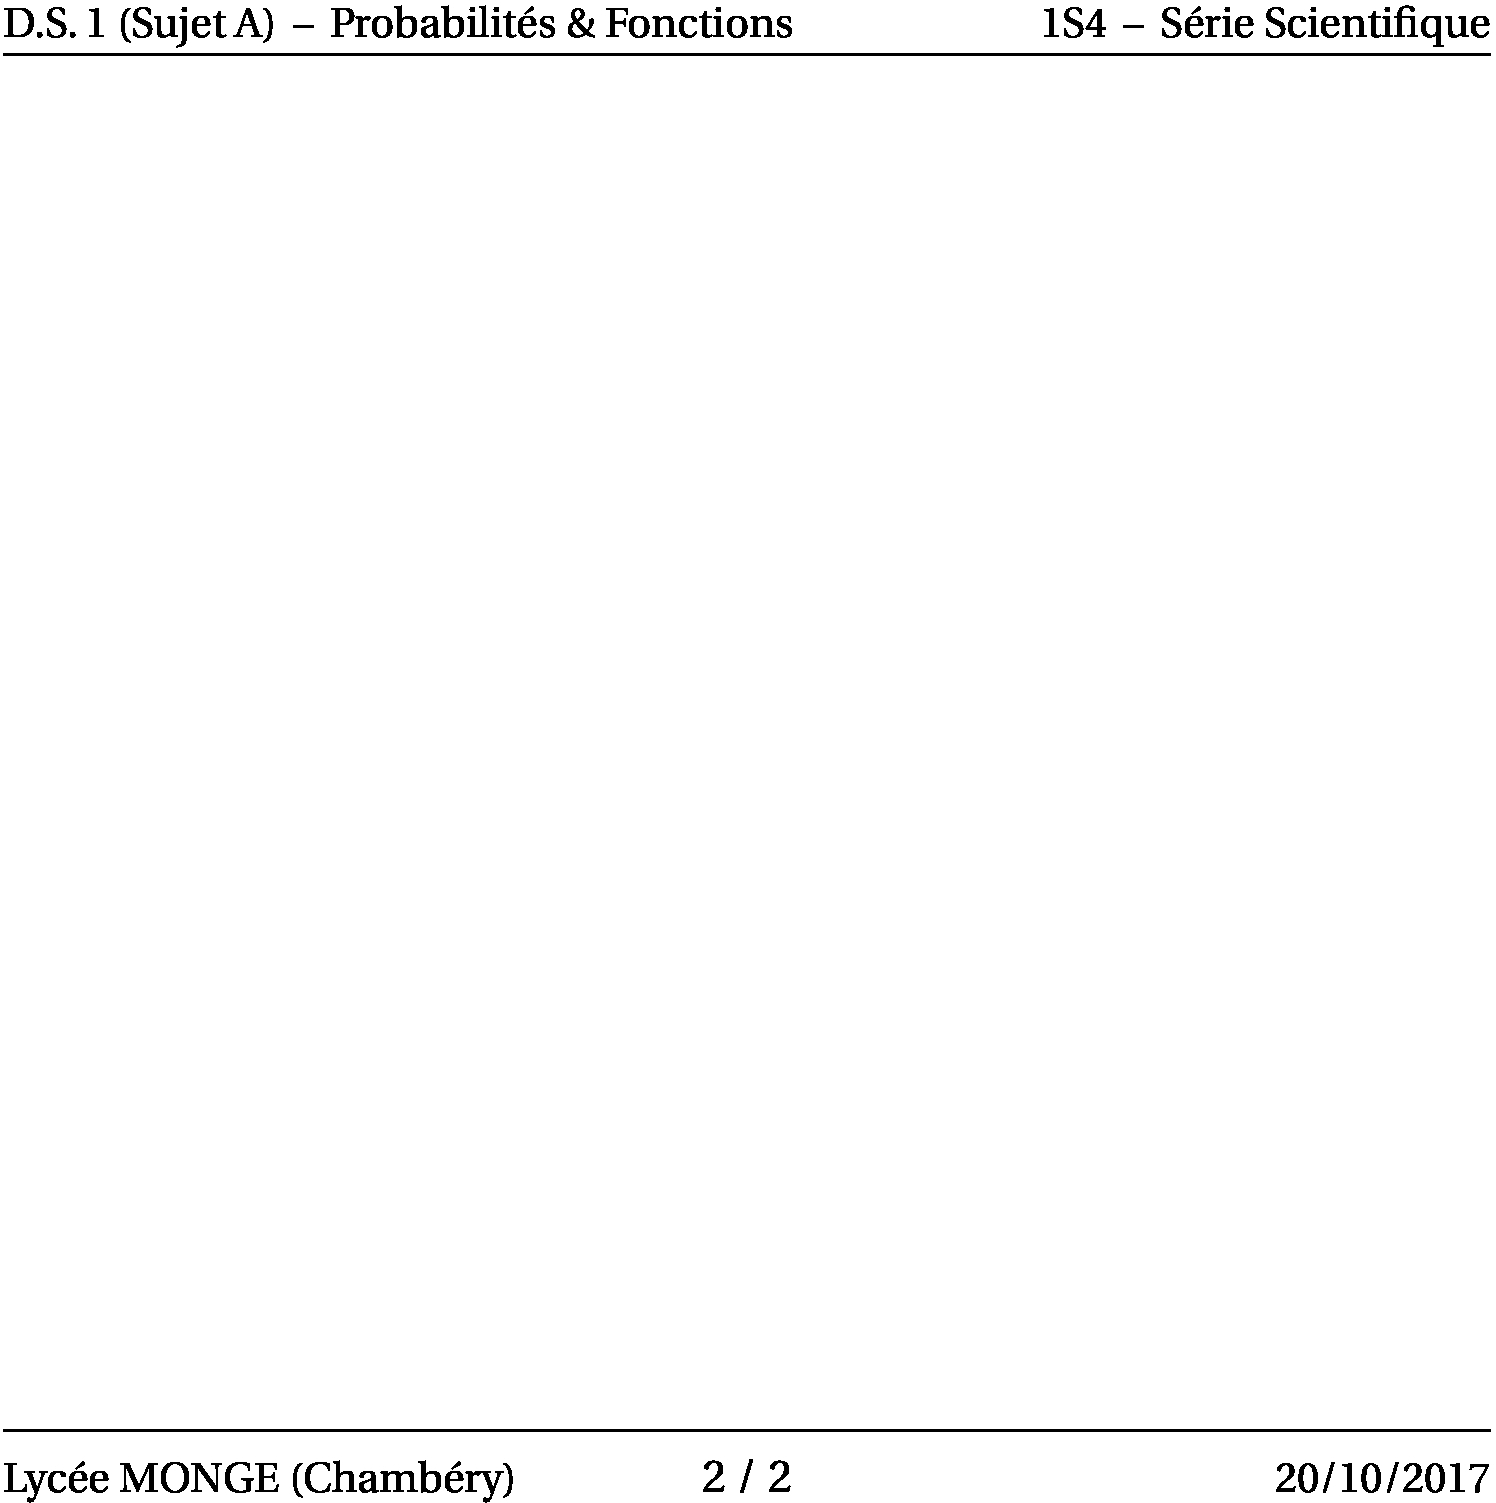
\includegraphics[width=0.9\linewidth]{example-doc[fr]-1.jpg}}
	\end{multicols}
\end{center}


Expliquons en détail le rôle de chacun des paramètres qui ont tous des valeurs de type texte \emph{(comme c'est toujours le cas, ou presque, avec \LaTeX{})}.

\begin{enumerate}
	\item \verb+kind+, \emph{qui doit obligatoirement être renseigné}, est tout simplement le type de devoir : un \emph{"D.S."}, un \emph{"D.M."}, une \emph{"Interrogation Surprise"}, une \emph{"Fiche d'entraînement"}, une \emph{"Activité"}...
	Vous noterez que le terme \emph{"devoir"} ne se limite pas juste aux devoirs notés.

	\item \verb+render+ est à utiliser pour un sujet à rendre avec la copie : utiliser \verb+yes+ ou \verb+no+ pour \emph{"oui"} ou \emph{"non"}.
	Ceci a pour conséquence que le sujet débutera, ou non, par une zone où l'élève devra indiquer son nom et son prénom.

	\item \verb+nb+ porte bien son nom : c'est le numéro du devoir.

	\item \verb+subnb+ permet d'indiquer une sorte de numérotation secondaire. C'est utile par exemple pour indiquer \emph{"Sujet A"}, \emph{"Sujet B"} ...

	\item \verb+subject+ permet si besoin de donner la thématique générale du devoir comme par exemple \emph{"Mathématiques"}, \emph{"Informatique Générale"}...

	\item \verb+theme+ sert à compléter la thématique générale en indiquant un ou des points particuliers comme par exemple \emph{"Probabilités"}, \emph{"Réseaux"} ...

	\item \verb+sector+ sert à indiquer une section, au sens administratif, à laquelle s'adresse le devoir. Par exemple, pour un sujet de Bac S en France, on utiliserait \verb+sector = Série Scientifique+.

	\item \verb+class+ indique la classe et/ou le groupe auquel est destiné le devoir.

	\item \verb+location+ vous permet d'indiquer un lieu géographique, typiquement un établissement scolaire ou universitaire.

	\item \verb+date+ est pour la date du devoir.

	\item \verb+time+ est pour la durée du devoir.

	\item \verb+preambule+ vous aidera à indiquer un texte en préambule qui apparaîtra avant vos exercices pour par exemple rappeler des obligations légales ou bien des choses importantes.
	 Si vous avez besoin de faire des retours à la ligne dans votre préambule, vous avez deux possibilités :

	 \begin{enumerate}
		\item Le mieux est de définir une macro commande où vous taperez votre texte.

		\item Si vous ne savez pas comment créer une macro commande, vous pouvez simplement utiliser des accolades et \verb+\\+ pour chaque retour à la ligne comme par exemple dans \verb+preambule = {Ligne 1\\Ligne 2\\Ligne 3}+.
	\end{enumerate}
\end{enumerate}


	\subsection{Différentes mises en forme}

Le package est fourni avec des exemples de fichiers \LaTeX{} afin d'observer ce que permet \verb+lyxam+. Explorez-les !


	\subsection{Fiche technique}

\IDmacro{exam}{12}{0}

\IDkey{kind} le type de devoir. \emph{Ceci ne peut pas être un texte vide.}

\IDkey{render} pour un sujet à rendre, ou non, avec une zone pour le nom et le prénom de l'étudiant. Deux valeurs possibles : \verb+yes+ ou \verb+no+ (valeur par défaut).

\IDkey{nb} le numéro du devoir.

\IDkey{subnb} une numérotation secondaire du devoir.

\IDkey{subject} la matière, le sujet du devoir.

\IDkey{theme} un sous-thème ou une sous-partie de la matière ou du sujet du devoir.

\IDkey{sector} un secteur, une section, au sens administratif, à laquelle s'adresse le devoir.

\IDkey{class} la classe concernée par le devoir.

\IDkey{location} le lieu géographique où a lieu le devoir.

\IDkey{date} le texte donnant la date du devoir.

\IDkey{time} le texte indiquant juste la durée du devoir.

\IDkey{preambule} un texte en préambule du devoir pour rappeler des obligations légales ou bien des choses importantes.




\newcommand\exosoptions{
\IDkey{pts} le nombre de points avec le cas particulier de $0$ qui demande d'afficher "Non noté".

\IDkey{time} la durée de l'exercice.

\IDkey{id} un texte de votre choix pour remplacer le numéro (ceci a pour effet de bloquer temporairement la numérotation).

\IDkey{title} un titre.

\IDkey{note} une petite indication liée à l'exercice (comme par exemple qu'il ne s'adresse qu'aux élèves motivés).

\IDkey{src} la source utilisée pour confectionner l'exercice.
}


\section{Indiquer vos exercices}

    \subsection{Important pour la suite}

Tous les exemples utilisés ci-dessous ont été obtenus en indiquant dans le préambule les options suivantes : \verb+\usepackage[apmep, fr]{lyxam}+.


    \subsection{Différents types d'exercices}

Voici l'ensemble des commandes disponibles pour indiquer un type d'exercice.

% All kind of level 2 contexts - START
\begin{itemize}[label=\textbullet]
\makeatletter
    \item \verb+\activity+ correspond à "\lyxam@text@activity{}".
    
    \item \verb+\bonus+ correspond à "\lyxam@text@bonus{}".
    
    \item \verb+\exercise+ correspond à "\lyxam@text@exercise{}".
    
    \item \verb+\mcq+ correspond à "\lyxam@text@mcq{}".
    
    \item \verb+\praticalwork+ correspond à "\lyxam@text@praticalwork{}".
    
    \item \verb+\problem+ correspond à "\lyxam@text@problem{}".
\makeatother
\end{itemize}
% All kind of level 2 contexts - END

Dans la suite, nous donnerons des exemples principalement avec la commande \verb+\exercise+. Ceci n'est pas gênant car le principe reste identique pour les autres commandes.


    \subsection{Numérotation automatique "intelligente"}

En \textbf{compilant deux fois} au moins, \verb+lyxam+ va pouvoir donner une numérotation "intelligente" de vos exercices. Ci-dessous, on obtient classiquement des exercices tous numérotés où vous noterez que chaque type d'exercice a sa propre numérotation.


\begin{tcblisting}{}
\exercise
Bla, bla, bla, bla, bla, ...

\exercise
Bla, bla, bla, bla, bla, ...

\problem
Bla, bla, bla, bla, bla, ...

\problem
Bla, bla, bla, bla, bla, ...

\bonus
Bla, bla, bla, bla, bla, ...

\bonus
Bla, bla, bla, bla, bla, ...
\end{tcblisting}


Ci-dessous, il y a ce que l'on obtient si notre sujet ne contient qu'un seul problème et un seul bonus : pas besoin ici d'avoir un numéro pour ces derniers. C'est ce que fait \verb+lyxam+. Pas mal ! Non ?

\resetallcnt{}

\begin{tcblisting}{}
\exercise
Bla, bla, bla, bla, bla, ...

\exercise
Bla, bla, bla, bla, bla, ...

\problem
Bla, bla, bla, bla, bla, ...

\bonus
Bla, bla, bla, bla, bla, ...
\end{tcblisting}



    \subsection{Indiquer le barème}

La commande \verb+\exercise+ dispose de plusieurs options dont l'une permet de donner le nombre de points attribués à une exercice (en indiquant $0$ point, le package indiquera une exercice non noté : voir la section suivante pour un exemple). Voici comment indiquer un barème.

\resetallcnt{}

\begin{tcblisting}{}
\exercise[pts = 5]
Bla, bla, bla, bla, bla, ...

\exercise[pts = 15]
Bla, bla, bla, bla, bla, ...
\end{tcblisting}


    \subsection{Toutes les options en action}

Les fiches techniques données un peu plus bas expliquent le champs d'utilisation de chaque option.

\begin{tcblisting}{}
\exercise[pts   = 0,
          time  = 3 jours,
          id    = facultatif,
          title = Devinette,
          note  = Pour spécialistes uniquement,
          src   = Le livre des experts]
Bla, bla, bla, bla, bla, ...
\end{tcblisting}



    \subsection{Cacher le texte "Exercice"}

La version étoilée \verb+\exercise*+ permet de cacher le contexte qui du point de vue de \verb+lyxam+ sera ici le texte "Exercice". Ceci est surtout pratique pour les sous-parties présentées un peu plus bas. Dans ce genre de situation, il faut obligatoirement donner un titre.

\begin{tcblisting}{}
\exercise*[title = Juste mon titre]

Bla, bla, bla, bla, bla, ...
\end{tcblisting}

    \subsection{Fiches techniques}

Toutes les options données ci-dessous sont facultatives.

\bigskip


% IDmacro - All kind of level 2 contexts - START
\IDmacro{activity}{6}{0}

\IDmacro{bonus}{6}{0}

\IDmacro{exercise}{6}{0}

\IDmacro{mcq}{6}{0}

\IDmacro{praticalwork}{6}{0}

\IDmacro{problem}{6}{0}
% IDmacro - All kind of level 2 contexts - END

\exosoptions{}



\section{Indiquer des sous-parties dans vos exercices}

    \subsection{Un exemple suffit\dots{} ou presque}

La commande \verb+\subpart+, qui possède les mêmes options que les commandes de type exercice, permet d'indiquer des sous-parties dans un exercice. La numérotation des sous-parties est remise à zéro à chaque nouvelle utilisation d'une commande de type exercice comme le montre l'exemple suivant.

\resetallcnt{}

\begin{tcblisting}{}
\exercise

\subpart
Bla, bla, bla, bla, bla, ...

\subpart
Bla, bla, bla, bla, bla, ...


\exercise

\subpart
Bla, bla, bla, bla, bla, ...

\subpart
Bla, bla, bla, bla, bla, ...
\end{tcblisting}


    \subsection{Fiche technique}

Toutes les options données ci-dessous sont facultatives et identiques à celles vues précédemment.

\bigskip


% IDmacro - All kind of level 3 contexts - START
\IDmacro{subpart}{6}{0}
% IDmacro - All kind of level 3 contexts - END

\exosoptions{}



\section{Regrouper vos exercices par thèmes}

    \subsection{Un exemple suffit\dots{} ou presque}

La commande \verb+\topic+, qui possède les mêmes options que les commandes de type exercice, sert juste à regrouper des exercices par thématiques : fût un temps où dans les brevets du collège, il y avait une partie numérique et une autre géométrique.
Chaque nouvelle utilisation de \verb+\topic+ remet juste à zéro la numérotation des sous-parties, et non celles des contextes de type exercice.

\resetallcnt{}

\resetallcnt{}

\begin{tcblisting}{}
\topic

\exercise
Bla, bla, bla, bla, bla, ...

\exercise
Bla, bla, bla, bla, bla, ...


\topic

\exercise
Bla, bla, bla, bla, bla, ...
\end{tcblisting}


    \subsection{Fiche technique}

Toutes les options données ci-dessous sont facultatives et identiques à celles vues précédemment.

\bigskip


% IDmacro - All kind of level 1 contexts - START
\IDmacro{topic}{6}{0}
% IDmacro - All kind of level 1 contexts - END

\exosoptions{}




\section{Historique}

All the changes are described inside the folders \verb+change_log+ : see the sources of \verb+lyxam+ on \verb+github+. Here we just give a very short history of \verb+lyxam+.

\begin{description}
	\setlength\itemsep{1em}

	\item[2017-11-03] First public version \verb+0.0.0-beta+ of the package.
\end{description}



\end{document}
